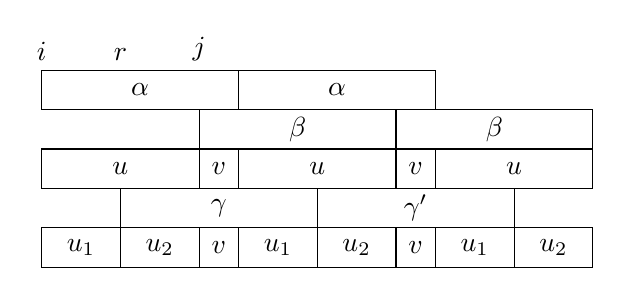
\begin{tikzpicture}[scale=0.5]
    %Facteur alpha beta, i,j
    \node[above] at (0,1) {$i$};
    \node[above] at (4,1) {$j$};
    \node[above] at (2,1) {$r$};
    \draw (0,0) rectangle (5,1) node[pos=.5] {$\alpha$};
    \draw (5,0) rectangle (10,1) node[pos=.5] {$\alpha$};
    \draw (4,0) rectangle (9,-1) node[pos=.5] {$\beta$};
    \draw (9,0) rectangle (14,-1) node[pos=.5] {$\beta$};
    %Facteur u,v,w
    \draw (0,-1) rectangle (4,-2) node[pos=.5] {$u$};
    \draw (4,-1) rectangle (5,-2) node[pos=.5] {$v$};
    \draw (5,-1) rectangle (9,-2) node[pos=.5] {$u$};
    \draw (9,-1) rectangle (10,-2) node[pos=.5] {$v$};
    \draw (10,-1) rectangle (14,-2) node[pos=.5] {$u$};
    %Mot intermédiaire
    \draw (2,-2) rectangle (7,-3) node[pos=.5] {$\gamma$};
    \draw (7,-2) rectangle (12,-3) node[pos=.5] {$\gamma'$};
    %Facteur u,v,w
    \draw (0,-3) rectangle (2,-4) node[pos=.5] {$u_1$};
    \draw (2,-3) rectangle (4,-4) node[pos=.5] {$u_2$};
    \draw (4,-3) rectangle (5,-4) node[pos=.5] {$v$};
    \draw (5,-3) rectangle (7,-4) node[pos=.5] {$u_1$};
    \draw (7,-3) rectangle (9,-4) node[pos=.5] {$u_2$};
    \draw (9,-3) rectangle (10,-4) node[pos=.5] {$v$};
    \draw (10,-3) rectangle (12,-4) node[pos=.5] {$u_1$};
    \draw (12,-3) rectangle (14,-4) node[pos=.5] {$u_2$};
\end{tikzpicture}